%
% Niniejszy plik stanowi przyk³ad formatowania pracy magisterskiej na
% Wydziale MIM UW.  Szkielet u¿ytych poleceñ mo¿na wykorzystywaæ do
% woli, np. formatujac wlasna prace.
%
% Zawartosc merytoryczna stanowi oryginalnosiagniecie
% naukowosciowe Marcina Wolinskiego.  Wszelkie prawa zastrze¿one.%
% Copyright (c) 2001 by Marcin Woliñski <M.Wolinski@gust.org.pl>
% Poprawki spowodowane zmianami przepisów - Marcin Szczuka, 1.10.2004
% Poprawki spowodowane zmianami przepisow i ujednolicenie 
% - Seweryn Kar³owicz, 05.05.2006
% dodaj opcjê [licencjacka] dla pracy licencjackiej
\documentclass{pracamgr}
  
  
  \usepackage[T1]{fontenc}
\usepackage[polish]{babel}
\usepackage[utf8]{inputenc}  
\usepackage[british,UKenglish,USenglish,english,american]{babel}
\usepackage{graphicx}
\usepackage[latin2]{inputenc}
 
%\usepackage[style=numeric,sorting=ydnt,defernumbers=true]{biblatex}
%	\DeclareFieldFormat{labelnumber}{\mkbibdesc{#1}}

%\makeatletter
%
%% Print labelnumber as actual number, plus item total, minus one
%\newrobustcmd{\mkbibdesc}[1]{%
%  \number\numexpr\csuse{bbx@itemtotal}+1-#1\relax}

% Initialize category counters
%\def\bbx@initcategory#1{\csnumgdef{bbx@count@#1}{0}}
%\forlistloop{\bbx@initcategory}{\blx@categories}
%
%% Increment category counters
%\def\bbx@countcategory#1{%
%  \ifentrytype{#1}
%    {\csnumgdef{bbx@count@#1}{\csuse{bbx@count@#1}+1}%
%     \addtocategory{#1}{\thefield{entrykey}}%
%     \listbreak}
%    {}}
%\AtDataInput{\forlistloop{\bbx@countcategory}{\blx@categories}}
%
%% Modify \bibbycategory to set item total
%\patchcmd{\blx@bibcategory}
%  {\blx@key@heading{#1}}
%  {\blx@key@heading{#1}%
%   \csnumdef{blx@labelnumber@\the\c@refsection}{0}%
%   \csnumgdef{bbx@itemtotal}{\csuse{bbx@count@#1}}}
%  {}{}
%
%\makeatother

%\DeclareBibliographyCategory{article}
%\DeclareBibliographyCategory{book}
%\DeclareBibliographyCategory{report}
%\DeclareBibliographyCategory{inproceedings}

%\defbibheading{article}{\subsection*{Journal Articles}}
%\defbibheading{book}{\subsection*{Books}}
%\defbibheading{report}{\subsection*{Reports}}
%\defbibheading{inproceedings}{\subsection*{Presentations}}
%\addbibresource{ref.bib}
%%Jesli uzywasz kodowania polskich znakow ISO-8859-2 nastepna linia powinna byc 
%odkomentowana
%Jesli uzywasz kodowania polskich znakow CP-1250 to ta linia powinna byc 
%odkomentowana
%\usepackage[cp1250]{inputenc}

% Dane magistranta:

\author{Konrad Lisiecki}
\nralbumu{48211}
\title{Stochastic Volatility Models}
\tytulang{haha}
\kierunek{Finanse i rachunkowo¶æ}
\instytut{Ekonometrii}
\opiekun{dra hab. £ukasza Delonga}
% miesi±c i~rok:
\date{Warsaw 2014}
%Podaæ dziedzinê wg klasyfikacji Socrates-Erasmus:
\dziedzina{  14.3 Ekonomia\\ }

%Klasyfikacja tematyczna wedlug AMS (matematyka) lub ACM (informatyka)
\klasyfikacja{D. Software\\
  D.127. haha\\
  D.127.6. Numerical blabalysis}

% S³owa kluczowe:
\keywords{haha}

% Tu jest dobre miejsce na Twoje w³asne makra i~¶rodowiska:
\newtheorem{defi}{Definicja}[section]

% koniec definicji 

%\makeindex[intoc]

















\begin{document}
\maketitle
\nocite{book-full}



 
\begin{abstract} 
sadfsdf
\end{abstract}

\tableofcontents






\chapter*{Wstep}

\begin{quote}

%   Alan White and I spent the next two or three years working together on this.
We developed what is known a stochastic volatility model. This is a model where the volatility as well as the underlying asset price moves around in an unpredictable way.

\raggedleft\slshape John Hull \index{Hull John}
\end{quote}

\addcontentsline{toc}{chapter}{Introduction} \markboth{INTRODUCTION}{} 
asdfsadf





\chapter{Wprowadzenie}\label{r:pojecia}
\begin{quote}

Never think that lack of variability is stability. Don't confuse lack of volatility with stability, ever.
 
\raggedleft\slshape Nassim Nicholas Taleb \index{Taleb Nassim Nicholas}
\end{quote}
 


adsafdsdfs
 
\section{Definicje}
dsfdsf

\begin{defi}\label{aa}
fsdf
\end{defi}

\begin{defi}\label{aaa}
sdfsdf
\end{defi}





\chapter{Model Hestona}
\begin{quote}
  Suppose we use the standard deviation ... of possible future returns on
  a stock ... as a measure of its volatility. Is it reasonable to take
  that volatility as a constant over time? I think not.

\raggedleft\slshape Fisher Black \index{Fisher, Black}
\end{quote}

Obecnie jednym z najpopularniejszych narzêdzi do wyceny opcji jest model Blacka-Scholsa. Ceniony jest on ze wzglêdu na prostotê oraz wygodê u¿ycia, kosztem jednak wielu upraszczaj±cych za³o¿eñ. Jednym z najwa¿niejszych jest za³o¿enia o sta³ej zmienno¶ci instrumentu bazowego, co w znacz±cym stopniu ogranicza precyzje oszacowañ. Jednym z pomys³ów na obej¶cie tego problemu jest uzmiennienie tej sta³ej, czyli pozwolanie, aby dla dowolnego czasu, parametr ten przyjmowa³ ró¿n± warto¶æ. Mo¿na to zrobiæ np. poprzez pozwolenie, aby nie tylko proces ceny akcji by³ procesem stochastycznym, ale tak¿e aby sama zmienno¶æ by³a niedetrministyczna, tzn. aby by³a równie¿ definiowana przy u¿yciu procesu stochastycznego. Takie te¿ podej¶cie zosta³o wykorzystane przy budowie modelu Hestona.

\section{Model Blacka-Scholesa}

Jak zostalo wspomniene we wstepie podstawowym modelem matematycznym na wycenê opcji jest model Blacka-Scholesa. Najczê¶ciej definiuje siê go w nastêpuj±cej postaci:
\begin{equation}
dS_t  = \mu S_t dt + \sigma S_t dW^S_t
\end{equation}

We wzorze tym $S_t$ przedstawia cenê instrumentu bazowego w momencie $t$, sta³a $\mu$ oznacza dryf, sta³a $\sigma$ oznacza zmienno¶æ, natomiast $dW^S_t$ jest standardowym procesem Wienera (procesem b³±dzenia losowego).


 

\section{Model Hestona}

Na pocz±tek za³ó¿my, ¿e cena aktywa bazowego w momemcie $t$ spe³nia nastêpuj±cy proces dyfuzji:
\begin{equation}
dS(t)= \mu S dt + \sqrt{v(t)} S d z_1 (t),
\end{equation}
gdzie $z_1(t)$  jest standardowym procesem Wienera. 

Je¿eli natomiast zmienno¶æ jest procesem Ornsteina-Uhlenbecka:

\begin{equation}
d \sqrt{v(t)} = - \beta \sqrt{v(t)} dt + \delta d z_2 (t)
\end{equation}

wtedy na podstawie lematu Ito mo¿na wykazaæ, ¿e wariancja $v(t)$ ma nastepuj±c± postaæ:
\begin{equation}
dv(t)= []dt+2\delta \sqrt{v(t)} d z_2 (t)
\end{equation}
gdzie proces $z_2(t)$ ma korelacjê z procesem $z_1(t)$ równ± $\rho$.

Gdy przyjmiemy sta³± stopê procentow±, cena w momencie $t$ obligacji, która wygasa w chwili $t+\tau$ wynosi:
\begin{equation}
P(t, t+\tau) = e^{-r\tau}
\end{equation}



\begin{figure}
  \centering
  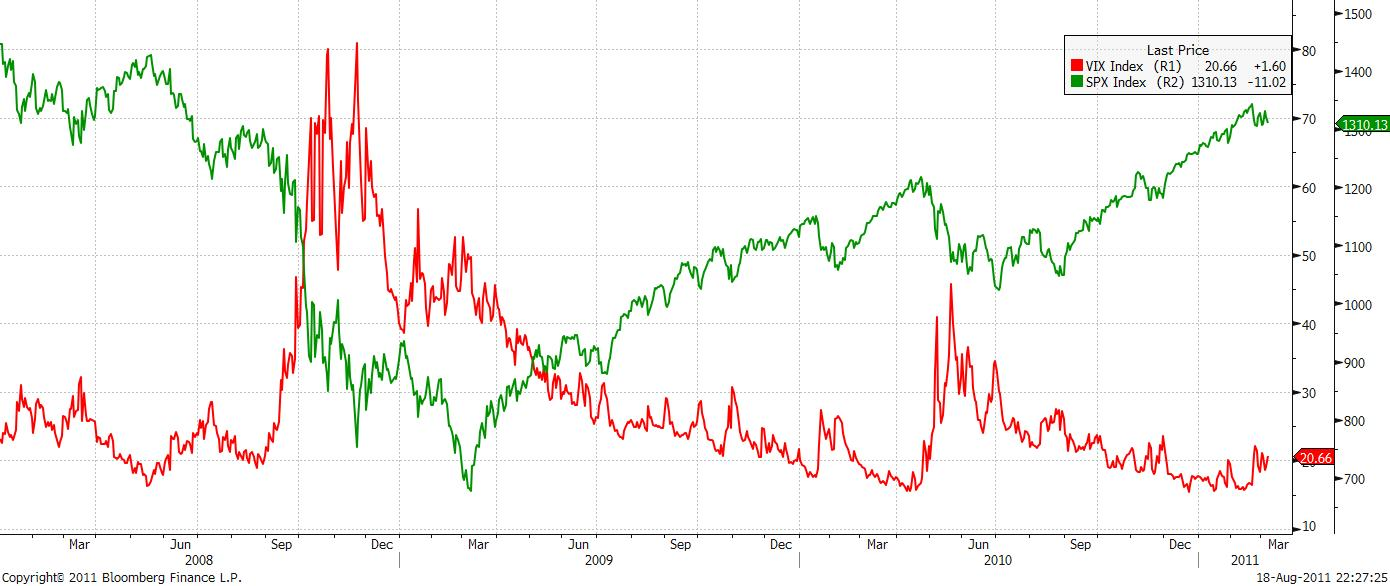
\includegraphics[width=150mm]{vix.jpg}
  \caption{Zmieno¶æ w czasie indeksu S\&P}\label{fig:vix}
\end{figure}


gdzie parametr $\sigma$ jest sta³y. Za³o¿enie to jednak okazujê siê byæ zbyt upraszczaj±ce dla szerokiej gamy szeregów czasowych. Spojrzmy np. na szereg czasowy  (\ref{fig:vix}) 



\begin{equation}\label{h:ito}
dv(t) = [\delta^2 - 2 \beta v(t)] dt + 2\beta \sqrt{v(t)} dz_2(t),
\end{equation}

The (\ref{h:ito}) equation can be rewritten to the following, square root process

\begin{equation}\label{h:squareroot}
dv(t) = \kappa [\theta - v(t)] dt + \sigma \sqrt{v(t)} d_2 (t),
\end{equation}

\chapter{Wycena opcji na indeks S\&P}\label{r:sp}
Lorem ipsum
 
 \chapter{Tematy dalszych studiów}\label{r:next}
Lorem ipsum
 \chapter*{Zakoñczenie}\label{r:ending}
Lorem ipsum



\appendix

%\chapter{Basic concepts and definitions}
%
%\begin{verbatim}
%[[foo]{,}[[a3,(([(,),{[[]]}]),
%  [1; [{,13},[[[11],11],231]]].
%  [13;[!xz]].
%  [42;[{,x},[[2],{'a'},14]]].
%  [br;[XQ*10]].
% ), 2q, for, [1,]2, [..].[7]{x}],[(((,[[1{{123,},},;.112]],
%        else 42;
%   . 'b'.. '9', [[13141],{13414}], 11),
% [1; [[134,sigma],22]].
% [2; [[rho,-],11]].
% )[14].
% ), {1234}],]. [map [cc], 1, 22]. [rho x 1]. {22; [22]},
%       dd.
% [11; sigma].
%        ss.4.c.q.42.b.ll.ls.chmod.aux.rm.foo;
% [112.34; rho];
%        001110101010101010101010101010101111101001@
% [22%f4].
% cq. rep. else 7;
% ]. hlt
%\end{verbatim}

%\chapter{Algorithm input data}
%
%\begin{center}
%  \begin{tabular}{rrr}
%    $\alpha$ & $\beta$ & $\gamma_7$ \\
%    901384 & 13784 & 1341\\
%    68746546 & 13498& 09165\\
%    918324719& 1789 & 1310 \\
%    9089 & 91032874& 1873 \\
%    1 & 9187 & 19032874193 \\
%    90143 & 01938 & 0193284 \\
%    309132 & $-1349$ & $-149089088$ \\
%    0202122 & 1234132 & 918324098 \\
%    11234 & $-109234$ & 1934 \\
%  \end{tabular}
%\end{center}

%\chapter{Exemplary results}
%
%\begin{center}
%  \begin{tabular}{lrrrr}
%    & Coefficients \\
%    & haha & $\rho$ & $\sigma$ & $\sigma$-$\rho$\\
%    $\gamma_{0}$ & 1,331 & 2,01 & 13,42 & 0,01 \\
%    $\gamma_{1}$ & 1,331 & 113,01 & 13,42 & 0,01 \\
%    $\gamma_{2}$ & 1,332 & 0,01 & 13,42 & 0,01 \\
%    $\gamma_{3}$ & 1,331 & 51,01 & 13,42 & 0,01 \\
%    $\gamma_{4}$ & 1,332 & 3165,01 & 13,42 & 0,01 \\
%    $\gamma_{5}$ & 1,331 & 1,01 & 13,42 & 0,01 \\
%    $\gamma_{6}$ & 1,330 & 0,01 & 13,42 & 0,01 \\
%    $\gamma_{7}$ & 1,331 & 16435,01 & 13,42 & 0,01 \\
%    $\gamma_{8}$ & 1,332 & 865336,01 & 13,42 & 0,01 \\
%    $\gamma_{9}$ & 1,331 & 34,01 & 13,42 & 0,01 \\
%    $\gamma_{10}$ & 1,332 & 7891432,01 & 13,42 & 0,01 \\
%    $\gamma_{11}$ & 1,331 & 8913,01 & 13,42 & 0,01 \\
%    $\gamma_{12}$ & 1,331 & 13,01 & 13,42 & 0,01 \\
%    $\gamma_{13}$ & 1,334 & 789,01 & 13,42 & 0,01 \\
%    $\gamma_{14}$ & 1,331 & 4897453,01 & 13,42 & 0,01 \\
%    $\gamma_{15}$ & 1,329 & 783591,01 & 13,42 & 0,01 \\
%  \end{tabular}
%\end{center}




\listoffigures
\addcontentsline{toc}{chapter}{List of figures} \markboth{Figures}{}
\listoftables
\addcontentsline{toc}{chapter}{List of tables} \markboth{Tables}{}

\chapter*{Bibliography}
\addcontentsline{toc}{chapter}{Bibliography} \markboth{Bibliography}{}

\begin{quote}
"Widzia³em dalej dziêki temu, ¿e sta³em na barkach gigantów".\\
%(If I have seen farther than others, it is because I was standing on the shoulders of giants).

\raggedleft\slshape Isaac Newton
\end{quote}

%\bibbycategory

%\printbibliography[category=article,title={Published Articles}]

%\printbibliography[category=articlepublished,title={Published Articles}]

%\printbibliography[category=articleunpublished,title={Unpublished Articles}]

%\printbibliography
%\printindex

\end{document}


%%% Local Variables:
%%% mode: latex
%%% TeX-master: t
%%% coding: latin-2
%%% End:
